\chapter{Conclusion \& Future Work}\label{chap:chap4}

\section{Conclusion}

In our preparation for dissertation we explored and presented the problem of software merges, more specifically, the difficulty in establishing an automated method to detect, identify and highlight semantic conflicts that arise.

We explored related work that can provide avenues of study and structures to guide the development of our solution. Specifically, previous work on test generation to identify semantic conflicts, the state of the art of automated test generation and the usage of Large Language Models for test generation, with specific focus on the important of appropriate prompting as well as output correction.

Forward, we will apply this knowledge in developing a solution that can hopefully aid developer workflows by identifying and generating tests for semantic conflicts.

\section{Future Work}

\subsection{Development Plan and Tool Functioning}

Development of the solution will go through several stages. Firstly, the process which has already been in progress, is the initial evaluation of LLM's and prompt techniques. After acquiring the list of subjects to test and deciding on the LLM, we can systematize this to develop the prototype solution. From here we start developing a tool that can automatically generate a prompt, get a test from the LLM and then run it. This prototype tool can then be further augmented, by applying corrections for tests that may fail to compile. \Cref{fig:tool} details the expected functioning of the tool once completed. A final period of evaluation and observations will compare our results to previous work and reflect on possible further improvements.

\begin{figure}
    \centering
    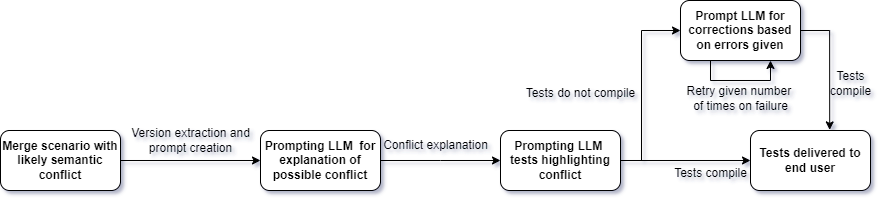
\includegraphics[width=1\linewidth]{figures/tool.png}
    \caption{Functioning pipeline of proposed tool}
    \label{fig:tool}
\end{figure}

\begin{figure}
    \centering
    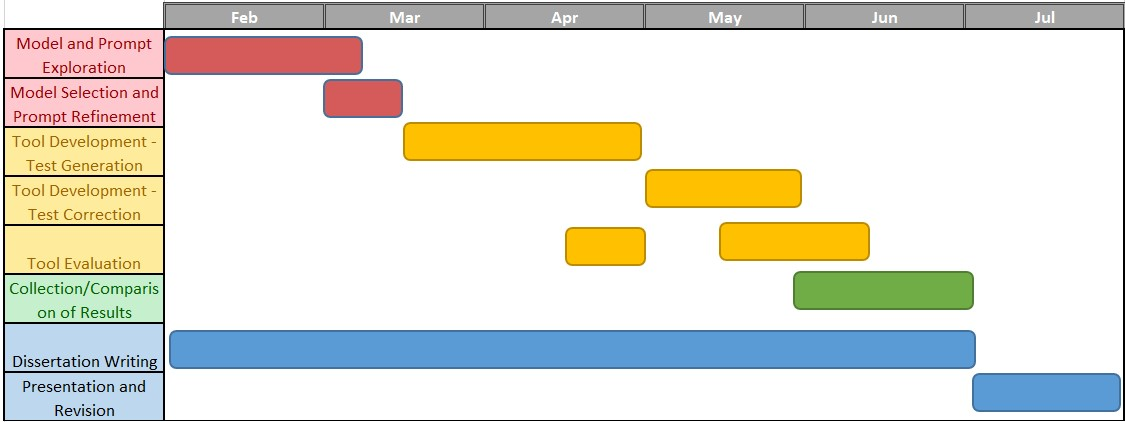
\includegraphics[width=1\linewidth]{figures/gantt.jpg}
    \caption{Gantt diagram of working plan}
    \label{fig:gantt}
\end{figure}
